% small.tex
\RequirePackage{atbegshi} 
\documentclass{beamer}
\usetheme[height=7mm]{Rochester}

\usepackage{graphicx}
\usepackage{hyperref}
\usepackage{skull}
\usepackage{verbatim}

\begin{document}

\begin{frame}{Intro}

Motivation:
\begin{itemize}
\item Robot for Eurobot, etc.
\item Need robust platform to handle all tasks
\item Robust bus for communication among components
\end{itemize}

We chose:
\begin{itemize}
\item Beagleboard
\item Controller Area Network - CAN
\end{itemize}
\end{frame}

\begin{frame}{Beagleboard}
\begin{columns}[c]

\column{.4\textwidth}
:-)
\begin{itemize}
\item OMAP3530 - Cortex-A8, 600MHz, 128MB RAM/Flash,
\item 2x SPI bus 
\item 1x I2C bus 
\item SD-card slot
\item USB OTG
\item HDMI
\item many others, ...
\end{itemize}

:-(
\begin{itemize}
\item No RTC
\item No network connectivity
\end{itemize}

\column{.6\textwidth}
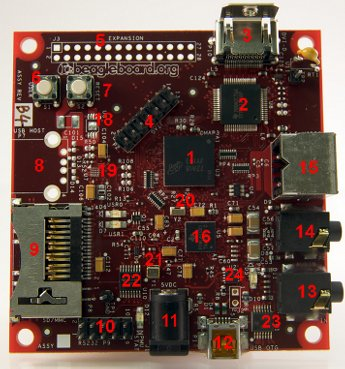
\includegraphics[width=\textwidth]{../img/beagleboard}

\end{columns}
\end{frame}

\begin{frame}{Expansion Board}
\centering{\includegraphics[height=.5\textheight]{../img/system}}
\begin{itemize}
\item Expands Beagleboard capabilities 
\item RTC with battery
\item 10/100Mbit Ethernet (ENC424J600)
\item STM32 MCU (Cortex-M3 based) \begin{itemize}
\item CAN bus
\item Battery/power management
\end{itemize}
\item Exposes more BB peripherals - UART, I2C
\end{itemize}
\end{frame}

\begin{frame}{What did we do}

\begin{columns}[c]
\column{.4\textwidth}

\begin{itemize}
  \item Ethernet driver
  \item Firmware for embedded MCU
  \item Counterpart driver for embedded MCU 
\end{itemize}

\column{.6\textwidth}
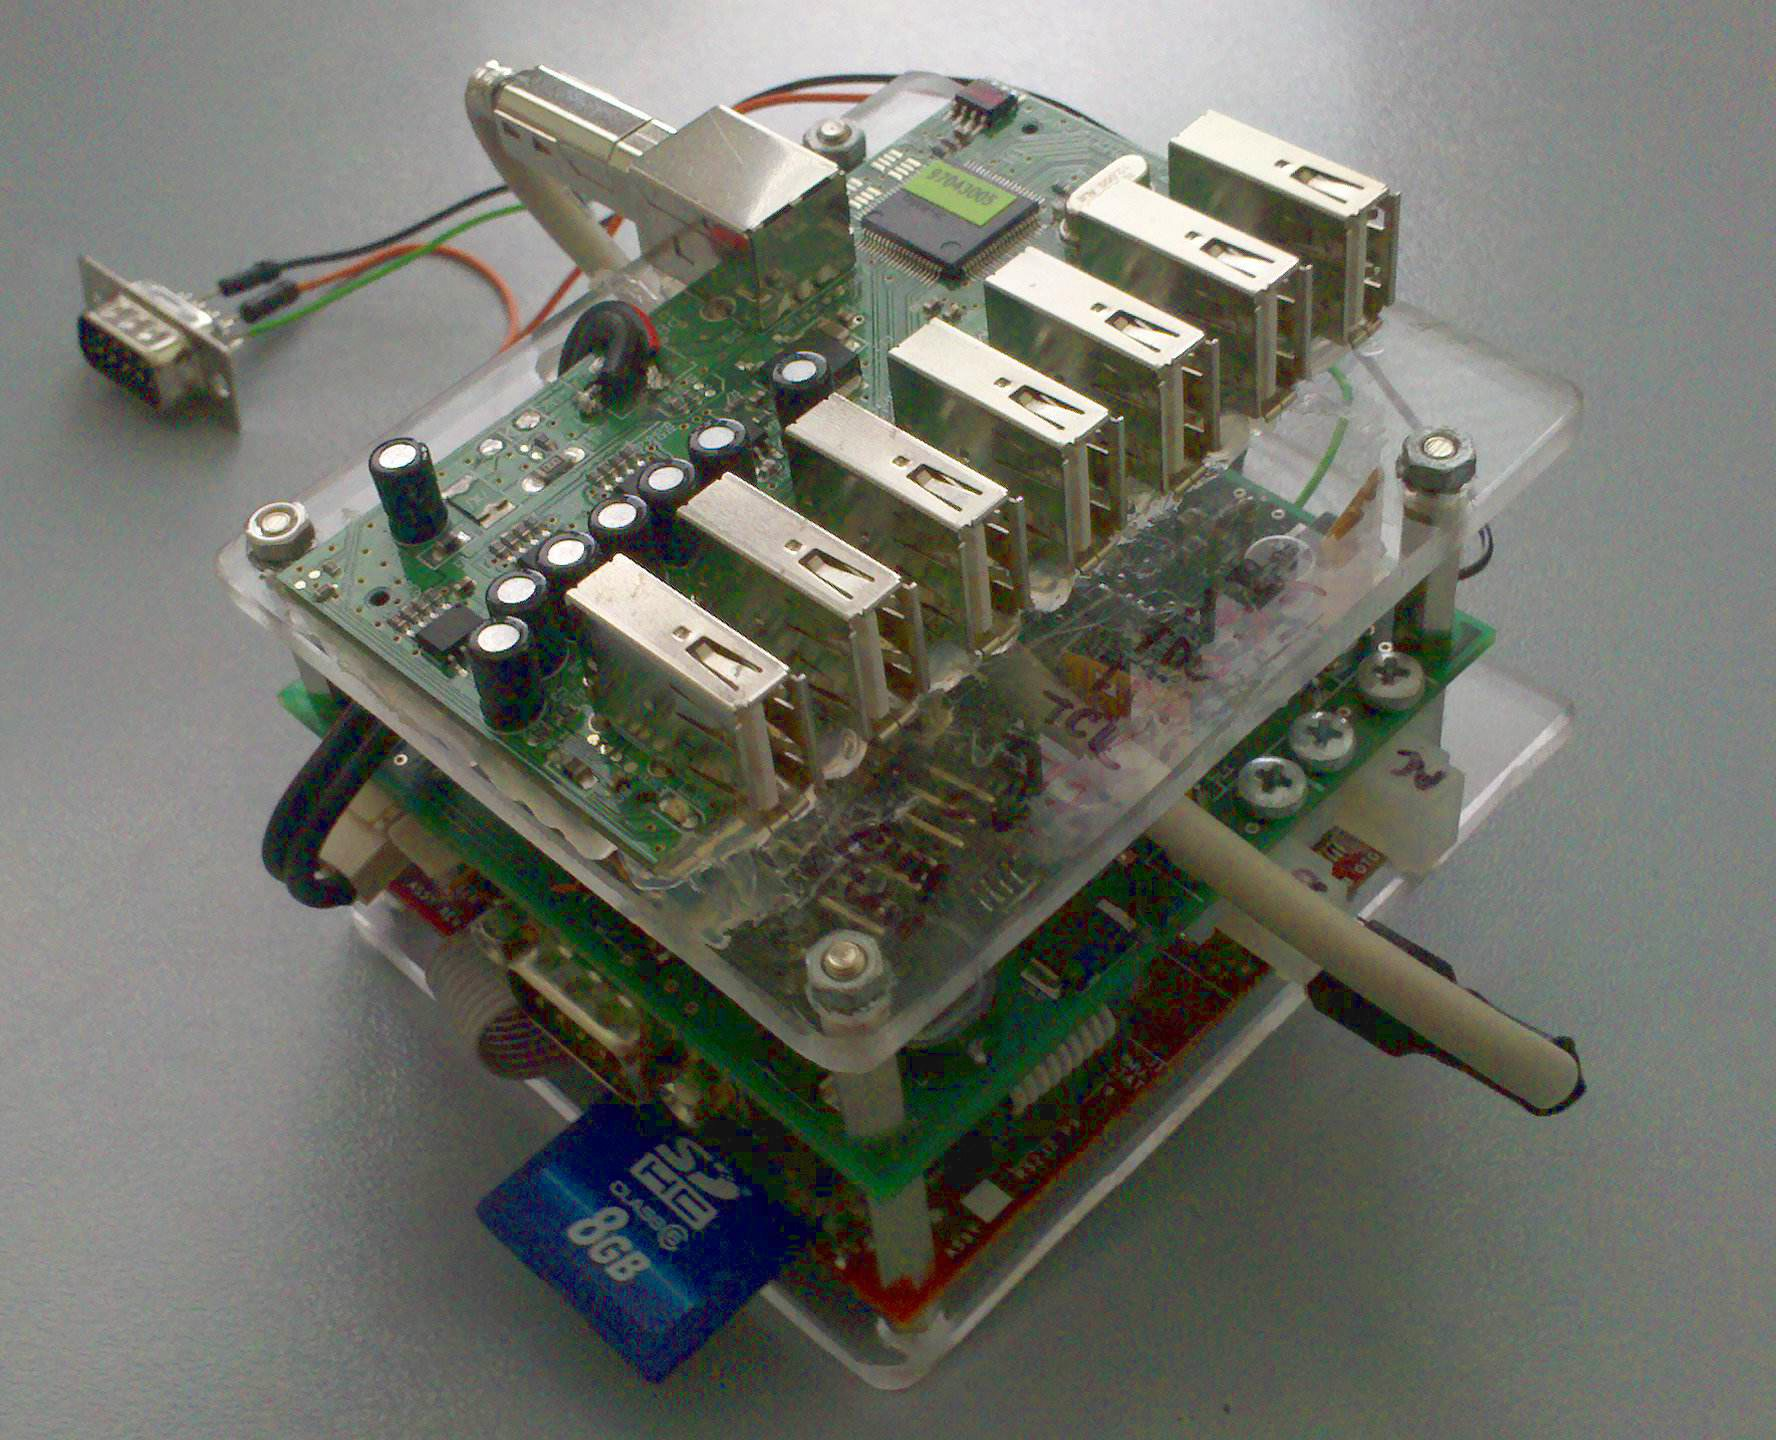
\includegraphics[width=\textwidth]{../img/main}

\end{columns}
\end{frame}

\begin{frame}{Ethernet - ENC424J600}
\begin{itemize}
  \item Straightforward implementation
	\item HW designed explicitly for embedded devices.
	\item Missing some features (atomic read'n'clear, ...)
\end{itemize}

\begin{itemize}
\item Developed on stable 2.6.29 kernel
\item During writing driver got forked by Indian programmer (and rejected from mainline kernel) :-)
\end{itemize}
\end{frame}

\begin{frame}{Ethernet - ENC424J600}
\begin{itemize}
	\item Working autonegotiation, 100/10Mbit, full/half duplex, low-power mode
	\item UDP throughput: ~12Mbit (up+down) 
	\item TCP throughput: ~2.5Mbit
\end{itemize}

\begin{itemize}
  \item Main bottleneck is SPI (14Mbit/s raw)
	\item Very slight improvement possible by preloading packets into ENCxxx chip
\end{itemize}
\end{frame}

\begin{frame}{Embedded MCU - SPI communication}
Protocol rewritten from scratch 2 times

Version 1:
\begin{itemize}
	\item 1 byte command + dummy byte + data
	\item dummy byte = time to process command
	\item Nested interrupts \(\skull\)
	\item Impossible to synchronize MCU with Beagleboard.
\end{itemize}

Version 2 - current:
\begin{itemize}
\item 1 byte command, ACK from MCU, then data
\item Added dedicated interrupt (GPIO) for ACK
\end{itemize}
\end{frame}

\begin{frame}{Embedded MCU - CAN}
\begin{itemize}
	\item Internal bxCAN hardware (3 message RX fifo, 3 TX mailboxes)
  \item Implements 16 message buffer, for message bursts 
	\item Fully interrupt based.
\end{itemize}

\begin{itemize}
\item Bug in HW causes false error reporting :-(
\item Possible speed improvement by preloading messages into TX mailboxes 
\end{itemize}
\end{frame}

\begin{frame}{Embedded MCU - Power}
\begin{itemize}
	\item Uses internal ADC to measure
	\begin{itemize}
		\item Battery voltage
		\item Battery current
		\item System current
		\item AC Power
	\end{itemize}
	\item Uses DMA transfer to offload CPU
	\item Uses PWM to set charging current
	\item Provides interrupts on Battery low, AC present
	\item Glitch-free AC \(\Leftrightarrow\) Battery switch
\end{itemize}
\end{frame}

\begin{frame}{Kernel counterpart driver}
\begin{itemize}
	\item CAN through SocketCAN (netdev)
	\item Power through Linux Power API
	\item Some additional features available only as /sys entry

	\item All communication through SPI
	\item Two interrupts - interrupt and data ack line

	\item CAN is available as network interface (ifconfig can0 up)
\end{itemize}
\end{frame}

\begin{frame}{U-boot}
\begin{itemize}
	\item Bootloader for ARM and other processors
	\item Initializes basic HW and sets up pin multiplexing
	\item Pin muxing changed to support our expansion board
	\item Careful when replacing! Leads to bricked HW
\end{itemize}
\end{frame}

\begin{frame}{Lessons learned}
\begin{itemize}
	\item Time time time :-)
	\item Nested interrupts are evil \(\skull\)
	\item Protocol design is crucial
	\item "Read and clear"
	\item GPIO\_148 is not GPIO\_149
\end{itemize}
\end{frame}

\begin{frame}{THE END.}
\centering{THE END}
\end{frame}

\end{document}
